\documentclass[tikz,border=3pt]{standalone}
\usetikzlibrary{arrows.meta}
\usepackage[utf8]{inputenc}

\begin{document}
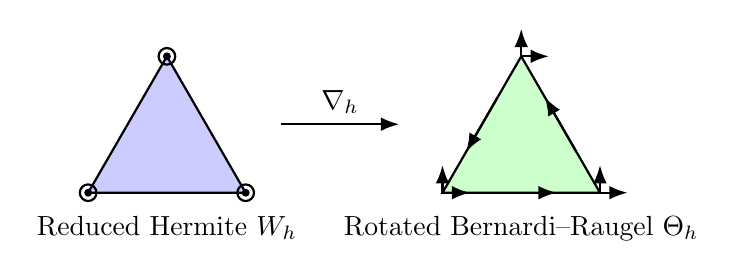
\begin{tikzpicture}[>=Latex]

  % Reduced cubic Hermite triangle: vertex values and Cartesian gradients.
  \begin{scope}[shift={(0,0)}]
    \filldraw[fill=blue!20, draw=black, thick]
      (0,0) -- (2,0) -- (1,1.732) -- cycle;
    % Filled dots show vertex values; hollow circles show the Cartesian gradient components.
    \foreach \p in {(0,0), (2,0), (1,1.732)} {
      \draw[fill=black, thick] \p circle (1pt);
      \draw[black, thick] \p circle (3pt);
    }
    \node at (1,-0.45) {Reduced Hermite $W_h$};
  \end{scope}

  % Discrete gradient operator.
  \draw[->, thick] (2.45,0.87) -- (3.95,0.87);
  \node at (3.2,1.15) {$\nabla_h$};

  % Rotated Bernardi--Raugel triangle: vertex vectors and tangent edge dofs.
  \begin{scope}[shift={(4.5,0)}]
    \filldraw[fill=green!20, draw=black, thick]
      (0,0) -- (2,0) -- (1,1.732) -- cycle;
    % The two vector degrees of freedom at each vertex follow the x and y axes.
    \draw[->, thick] (0,0) -- (0.35,0);
    \draw[->, thick] (0,0) -- (0,0.35);
    \draw[->, thick] (2,0) -- (2.35,0);
    \draw[->, thick] (2,0) -- (2,0.35);
    \draw[->, thick] (1,1.732) -- (1,2.082);
    \draw[->, thick] (1,1.732) -- (1.35,1.732);
    \draw[->, thick] (0.55,0) -- (1.45,0);
    \draw[->, thick] (1.70,0.52) -- (1.30,1.212);
    \draw[->, thick] (0.70,1.212) -- (0.30,0.52);
    \node at (1,-0.45) {Rotated Bernardi--Raugel $\Theta_h$};
  \end{scope}

\end{tikzpicture}
\end{document}
